% Do NOT change this "Section" title
% and do NOT add more "Section" level titles.
\section{Implementation}\label{sec:implementation}
Text

% You can use how many "subsections" and "subsubsections" you like.
\subsection{Subsection}
Text
\subsubsection{Subsubsection1}
Test of one column figure. It should be shown as close as possible to this
text. If you can't see the figure its number is \ref{fig:one_column_figure}
and located on page \pageref{fig:one_column_figure}.
\begin{figure}[h]
    
\includegraphics[width=0.5\textwidth]{./figure/figureA.png}
    \caption{Figure A}
    \label{fig:one_column_figure}
\end{figure}

\subsubsection{Subsubsection1}
Test of two columns figure. It should be shown at the top of a page. If you
can't see the figure its number is \ref{fig:two_column_figure}
and located on page \pageref{fig:two_column_figure}.
\begin{figure*}[t]
    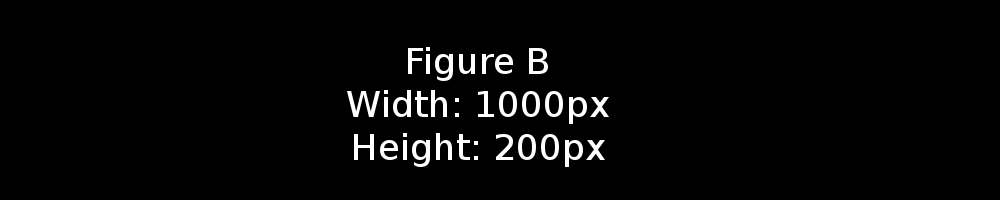
\includegraphics[width=1.0\textwidth]{./figure/figureB.png}
    \caption{Figure B}
    \label{fig:two_column_figure}
\end{figure*}
